\documentclass[0_main]{subfiles}

\begin{document}

\ifEn
    \section{Newton's Method}
\else
    \section{ニュートン法}
\fi
\label{sec:background_newton}

\ifEn
    \subsection{Algorithm of Newton's Method}
\else
    \subsection{ニュートン法のアルゴリズム}
\fi

\ifEn
    In this subsection, we outline Newton's method, which is a fundamental optimization algorithm for an unconstrained optimization problem.
    Newton's method is a representative iterative algorithm that starts from an initial point $x_0$, successively updates the current point, and generates a sequence $\{ x_k \}_{k=0}^\infty$.
\else
    本小節では、無制約最適化問題に対する基本的な最適化アルゴリズムであるニュートン法の概要を示す。
    ニュートン法は、初期点 $x_0$ から出発し、現在点を逐次更新して列 $\{ x_k \}_{k=0}^\infty$ を生成する代表的な反復アルゴリズムである。
\fi

\ifEn
    We assume that $f$ is of class $C^2$ and strongly convex, so that the Hessian matrix $\nabla^2 f(x)$ is positive definite for all $x \in \mathbb{R}^n$, and thus invertible.
    Using the gradient $g_k \coloneqq \nabla f(x_k)$ and Hessian $\nabla^2 f(x_k)$ at the $k$-th iterate $x_k$, the base procedure of Newton's method is to iteratively update
\else
    $f$ は $C^2$ 級で強凸であると仮定し、このときヘッセ行列 $\nabla^2 f(x)$ は任意の $x \in \mathbb{R}^n$ で正定値となり可逆である。
    $k$ 回目の反復点 $x_k$ における勾配 $g_k \coloneqq \nabla f(x_k)$ とヘッセ行列 $\nabla^2 f(x_k)$ を用いると、ニュートン法の基本手続きは次の更新を反復的に行うことである。
\fi
\begin{equation*}
    x_{k+1} \gets x_k - \alpha_k \nabla^2 f(x_k)^{-1} g_k
\end{equation*}
\ifEn
    with a step size $\alpha_k > 0$ determined by line search.
    The derivation of this update rule is as follows.
    The quadratic Taylor approximation of $f$ around $x_k$ is given by
\else
    ここで $\alpha_k > 0$ は線形探索によって定められるステップサイズである。
    この更新則の導出は次のとおりである。
    $x_k$ まわりの $f$ の二次のテイラー近似は次式で与えられる。
\fi
\begin{equation*}
    m^*_{k}(x) \coloneqq f(x_k) + g_k^\top (x - x_k) + \frac{1}{2} (x - x_k)^\top \nabla^2 f(x_k) (x - x_k).
\end{equation*}
\ifEn
    The gradient of this model is
\else
    このモデルの勾配は次式である。
\fi
\begin{equation*}
    \nabla m^*_k(x) = g_k + \nabla^2 f(x_k)(x - x_k).
\end{equation*}
\ifEn
    Since the quadratic model is strongly convex by assumption, a point $x^* \in \mathbb{R}^n$ is the minimizer of $m^*_k$ if and only if $\nabla m^*_k(x) = 0$. Thus, solving this equation yields
\else
    仮定よりこの二次モデルは強凸であるため、点 $x^* \in \mathbb{R}^n$ が $m^*_k$ の最小点であることと $\nabla m^*_k(x) = 0$ が成り立つことは同値である。したがって、この方程式を解くと次を得る。
\fi
\begin{equation*}
    \underset{x \in \mathbb{R}^n}{\mathrm{arg \ min}} \ m^*_{k}(x) = x_k -\left(\nabla^2 f(x_k)\right)^{-1} g_k.
\end{equation*}
\ifEn
    Although this choice appears natural, it does not in general guarantee global convergence, as we will see later.
    Thus, we introduce a step size $\alpha_k > 0$ determined by line search to ensure a sufficient decrease in the function value.
    This is the basic procedure of Newton's method.
\else
    この選択は自然に見えるが、後で見るように一般には大域収束を保証しない。
    そこで、関数値の十分な減少を確保するため、線形探索で定めるステップサイズ $\alpha_k > 0$ を導入する。
    これがニュートン法の基本手続きである。
\fi

\ifEn
    The update direction $d_k \coloneqq -\nabla^2 f(x_k)^{-1} g_k$ is known as the Newton direction, which is a descent direction when the Hessian is positive definite, since
\else
    更新方向 $d_k \coloneqq -\nabla^2 f(x_k)^{-1} g_k$ はニュートン方向と呼ばれる。ヘッセ行列が正定値であれば、次式より降下方向である。
\fi
\begin{equation*}
    g_k^\top d_k = -g_k^\top \nabla^2 f(x_k)^{-1} g_k < 0.
\end{equation*}
\ifEn
    If $f$ is nonconvex and the Hessian $\nabla^2 f(x_k)$ is negative definite or indefinite, function values are not guaranteed to decrease, and Newton's method may fail to converge.
    Therefore, checking the positive definiteness of the Hessian is important when applying Newton's method.
    The modified Newton method \citep[Sec. 3.4]{nocedal1999numerical} is one remedy for handling such cases.
\else
    $f$ が非凸であり、ヘッセ行列 $\nabla^2 f(x_k)$ が負定値または不定値である場合、関数値の減少は保証されず、ニュートン法は収束しないことがある。
    したがって、ニュートン法の適用ではヘッセ行列の正定値性の確認が重要である。
    このような場合への一つの対処法として修正ニュートン法 \citep[Sec. 3.4]{nocedal1999numerical} がある。
\fi

\ifEn
    \subsection{Properties Related to Convergence}
\else
    \subsection{収束に関する性質}
\fi
\label{sec:newton-local-convergence}
\ifEn
    We next present a standard convergence theorem for Newton's method.
\else
    次に、ニュートン法に対する標準的な収束定理を示す。
\fi

\ifEn
    \subsubsection{Global Convergence}
\else
    \subsubsection{大域収束}
\fi

\ifEn
    We first state a general global convergence result
\else
    まず、一般的な大域収束の結果
\fi
\begin{equation*}
    \lim_{k \to \infty} \lVert g_k \rVert = 0
\end{equation*}
\ifEn
    for methods with line search, and then explain its application to Newton's method.
    We consider a general iterative method of the form
\else
    を線形探索付きの手法に対して述べ、その後にニュートン法への適用を説明する。
    次の形の一般的な反復法を考える。
\fi
\begin{equation*}
    x_{k+1} \gets x_k + \alpha_k d_k,
\end{equation*}
\ifEn
    where $d_k$ is a descent direction satisfying $g_k^\top d_k < 0$ and $\alpha_k > 0$ is the step size determined by line search.
    We employ the Wolfe conditions \citep[Sec. 3.1]{nocedal1999numerical} to determine the step size $\alpha_k$ as follows:
\else
    ここで $d_k$ は $g_k^\top d_k < 0$ を満たす降下方向であり、$\alpha_k > 0$ は線形探索で決定されるステップサイズである。
    ステップサイズ $\alpha_k$ は Wolfe 条件 \citep[Sec. 3.1]{nocedal1999numerical} により次のように定める。
\fi
\begin{align*}
    f(x_k + \alpha_k d_k) & \leq f(x_k) + c_1 \alpha_k g_k^\top d_k, \\
    g_{k+1}^\top d_k      & \geq c_2 g_k^\top d_k,
\end{align*}
\ifEn
    where $0 < c_1 < c_2 < 1$ are constants.
    We also define $\theta_k \in [0, \pi]$ as the angle between the direction $d_k$ and the negative gradient $-g_k$, satisfying
\else
    ここで $0 < c_1 < c_2 < 1$ は定数である。
    また、方向 $d_k$ と負の勾配 $-g_k$ のなす角を $\theta_k \in [0, \pi]$ とし、次式を満たすように定める。
\fi
\begin{equation*}
    \cos \theta_k = \frac{-g_k^\top d_k}{\lVert g_k \rVert\lVert d_k \rVert}.
\end{equation*}
\ifEn
    The following theorem is a simplified version of the classical result.
\else
    次の定理は古典的結果の簡略版である。
\fi

\begin{theorem}[{\cite[Theorem 3.2]{nocedal1999numerical}}]
    \label{thm:line-search-global-convergence}
    \ifEn
        Suppose that $f$ is of class $C^1$ and bounded below in $\mathbb{R}^n$, and $L$-smooth.
        Consider the iterative method defined by
    \else
        $f$ は $C^1$ 級であり $\mathbb{R}^n$ 上で下に有界で、かつ $L$-平滑であるとする。
        次の反復法を考える。
    \fi
    \begin{equation*}
        x_{k+1} \gets x_k + \alpha_k d_k,
    \end{equation*}
    \ifEn
        starting from an initial point $x_0 \in \mathbb{R}^n$, and the step size $\alpha_k$ is determined by the Wolfe conditions.
        For the angle $\theta_k$, if there exists a positive constant $\delta$ such that
        $\cos \theta_k \geq \delta > 0$ for all $k$,
        then, the method generates a sequence $\{ x_k \}$ satisfying
    \else
        初期点 $x_0 \in \mathbb{R}^n$ から開始し、ステップサイズ $\alpha_k$ は Wolfe 条件で定められるとする。
        角 $\theta_k$ に対して、ある正の定数 $\delta$ が存在して
        $\cos \theta_k \geq \delta > 0$ がすべての $k$ で成り立つならば、
        この反復法は次を満たす列 $\{ x_k \}$ を生成する。
    \fi
    \begin{equation*}
        \lim_{k \to \infty} \lVert g_k \rVert = 0.
    \end{equation*}
\end{theorem}
\begin{proof}
    \ifEn
        From the Wolfe condition, we have
    \else
        Wolfe 条件より次が成り立つ。
    \fi
    \begin{equation*}
        (g_{k+1} - g_k)^\top d_k
        = g_{k+1}^\top d_k - g_k^\top d_k
        \geq (c_2 - 1) g_k^\top d_k,
    \end{equation*}
    \ifEn
        and
    \else
        また
    \fi
    \begin{align*}
        (g_{k+1} - g_k)^\top d_k                      & \leq
        \lVert g_{k+1} - g_k \rVert \lVert d_k \rVert &                                                      & \text{(Cauchy--Schwarz inequality)}                           \\
                                                      & \leq L \lVert x_{k+1} - x_k \rVert \lVert d_k \rVert &                                     & \text{($L$-smoothness)} \\
                                                      & = \alpha_k L \lVert d_k \rVert^2.
    \end{align*}
    \ifEn
        By combining these two relations, we obtain
    \else
        これらを組み合わせると次を得る。
    \fi
    \begin{equation*}
        \alpha_k \geq \frac{c_2 - 1}{L} \frac{g_k^\top d_k}{\lVert d_k \rVert^2},
    \end{equation*}
    \ifEn
        and thus
    \else
        よって
    \fi
    \begin{align*}
        f(x_{k+1}) & \leq f(x_k) + c_1 \alpha_k g_k^\top d_k                                          &  & \text{(Wolfe condition)}          \\
                   & \leq f(x_k) - c_1 \frac{1 - c_2}{L} \frac{(g_k^\top d_k)^2}{\lVert d_k \rVert^2} &  & \text{(previous inequality)}      \\
                   & = f(x_k) - c_1 \frac{1 - c_2}{L} \cos^2 \theta_k \lVert g_k \rVert^2.            &  & \text{(definition of $\theta_k$)}
    \end{align*}
    \ifEn
        By summing this expression over all indices less than or equal to $k$, we obtain
    \else
        この式を $k$ 以下のすべての添字について和を取ると次を得る。
    \fi
    \begin{equation*}
        f(x_{k+1}) \leq f(x_0) - c_1 \frac{1 - c_2}{L} \sum_{j=0}^k \cos^2 \theta_j \lVert g_j \rVert^2.
    \end{equation*}
    \ifEn
        Since $f$ is bounded below, we have that $f(x_0) - f(x_{k+1})$ is less than some positive constant for all $k$.
        Hence, by taking limits, we obtain the Zoutendijk condition:
    \else
        $f$ は下に有界なので、$f(x_0) - f(x_{k+1})$ はすべての $k$ である正の定数より小さい。
        したがって、極限を取ることで Zoutendijk 条件が得られる。
    \fi
    \begin{equation*}
        \sum_{k=0}^\infty \cos^2 \theta_k \lVert g_k \rVert^2 < \infty.
    \end{equation*}
    \ifEn
        This condition implies that
    \else
        この条件は次を含意する。
    \fi
    \begin{equation*}
        \cos^2 \theta_k \lVert g_k \rVert^2 \to 0.
    \end{equation*}
    \ifEn
        Combined with the assumption that $\cos \theta_k \geq \delta > 0$ for all $k$, it follows immediately that
    \else
        $\cos \theta_k \geq \delta > 0$ がすべての $k$ で成り立つという仮定と合わせると、直ちに次が従う。
    \fi
    \begin{equation*}
        \lim_{k \to \infty} \lVert g_k \rVert = 0,
    \end{equation*}
    \ifEn
        which completes the proof.
    \else
        これで証明が完了する。
    \fi
\end{proof}

\ifEn
    Since Newton's method is a special case of the setting in \cref{thm:line-search-global-convergence} with $d_k = -\nabla^2 f(x_k)^{-1} g_k$, we can apply this result under appropriate conditions of $f$.
    In particular, if $f$ is $L$-smooth and $\mu$-strongly convex, then for any $k$, we have
\else
    ニュートン法は $d_k = -\nabla^2 f(x_k)^{-1} g_k$ とした \cref{thm:line-search-global-convergence} の特別な場合なので、$f$ の適切な条件のもとでこの結果を適用できる。
    特に $f$ が $L$-平滑かつ $\mu$-強凸であれば、任意の $k$ について次が成り立つ。
\fi
\begin{equation*}
    \cos \theta_k
    = \frac{g_k^\top \nabla^2 f(x_k)^{-1} g_k}{\lVert g_k \rVert\lVert \nabla^2 f(x_k)^{-1} g_k \rVert}
    \geq \frac{\lVert g_k \rVert^2 \lambda_{\min}(\nabla^2 f(x_k)^{-1})}{\lVert g_k \rVert^2 \lambda_{\max}(\nabla^2 f(x_k)^{-1})}
    \geq \frac{\mu}{L},
\end{equation*}
\ifEn
    where $\lambda_{\min}(\cdot)$ and $\lambda_{\max}(\cdot)$ denote the minimum and maximum eigenvalues, respectively.
    Thus, by setting $\delta = \mu / L$ in \cref{thm:line-search-global-convergence}, we obtain the global convergence of Newton's method for strongly convex and smooth functions under line search satisfying the Wolfe conditions.
\else
    ここで $\lambda_{\min}(\cdot)$ と $\lambda_{\max}(\cdot)$ はそれぞれ最小固有値と最大固有値を表す。
    したがって、\cref{thm:line-search-global-convergence} において $\delta = \mu / L$ とすれば、Wolfe 条件を満たす線形探索のもとで、強凸かつ平滑な関数に対するニュートン法の大域収束が得られる。
\fi

\ifEn
    \subsubsection{Local Quadratic Convergence}
\else
    \subsubsection{局所二次収束}
\fi

\ifEn
    We next present a classical result on the local convergence rate of Newton's method.
    We again provide a simplified version for brevity as follows.
\else
    次に、ニュートン法の局所収束速度に関する古典的結果を示す。
    ここでも簡潔さのために簡略版を示す。
\fi

\begin{theorem}[{\cite[Theorem 3.5]{nocedal1999numerical}}]
    \label{thm:newton-quadratic}
    \ifEn
        Suppose that the Hessian matrix $\nabla^2 f(x)$ is Lipschitz continuous in a neighborhood of the solution $x^*$, and that sufficient second-order optimality conditions hold (i.e., $\nabla f(x^*)=0$ and $\nabla^2 f(x^*)$ is positive definite).
        If $\alpha_k=1$ for all $k$ and the initial point $x_0$ is sufficiently close to $x^*$,
        then the sequence of gradient norms $\{\lVert \nabla f(x_k) \rVert\}$ converges quadratically.
    \else
        ヘッセ行列 $\nabla^2 f(x)$ が解 $x^*$ の近傍で Lipschitz 連続であり、十分な二次の最適性条件が成り立つとする。すなわち $\nabla f(x^*)=0$ かつ $\nabla^2 f(x^*)$ は正定値である。
        すべての $k$ で $\alpha_k=1$ とし、初期点 $x_0$ が $x^*$ に十分近いとき、勾配ノルム列 $\{\lVert \nabla f(x_k) \rVert\}$ は二次収束する。
    \fi
\end{theorem}
\begin{proof}
    \ifEn
        From the definition of the Newton step and the optimality condition $\nabla f(x^*)=0$, we obtain
    \else
        ニュートンステップの定義と最適性条件 $\nabla f(x^*)=0$ より次を得る。
    \fi
    \begin{align*}
        x_{k+1} - x^*
         & = x_k - x^* - \left(\nabla^2 f(x_k)\right)^{-1}\nabla f(x_k)                                                        \\
         & = \left(\nabla^2 f(x_k)\right)^{-1} \left(\nabla^2 f(x_k)(x_k-x^*)-\left(\nabla f(x_k)-\nabla f(x^*)\right)\right).
    \end{align*}
    \ifEn
        By Taylor's theorem and the triangle inequality, we have
    \else
        テイラーの定理と三角不等式より次が成り立つ。
    \fi
    \begin{align*}
                & \lVert \nabla^2 f(x_k)(x_k-x^*)-\left(\nabla f(x_k)-\nabla f(x^*)\right) \rVert                    \\
        =   {}  & \lVert \nabla^2 f(x_k)(x_k-x^*)-\int_0^1 \nabla^2 f(x_k+t(x^*-x_k)) (x_k - x^*)\mathrm{d}t \rVert  \\
        \leq {} & \int_0^1 \lVert \nabla^2 f(x_k)-\nabla^2 f(x_k+t(x^*-x_k)) \rVert\lVert x_k-x^* \rVert\mathrm{d}t.
    \end{align*}
    \ifEn
        If $\nabla^2 f$ is Lipschitz continuous with constant $L^{\mathrm{H}}$, then the integrand is bounded by $L^{\mathrm{H}}t\lVert x_k-x^* \rVert$, and integrating yields
    \else
        $\nabla^2 f$ が定数 $L^{\mathrm{H}}$ を持つ Lipschitz 連続であれば、被積分関数は $L^{\mathrm{H}}t\lVert x_k-x^* \rVert$ で上から抑えられ、積分により次を得る。
    \fi
    \begin{equation*}
        \lVert \nabla^2 f(x_k)(x_k-x^*)-\left(\nabla f(x_k)-\nabla f(x^*)\right) \rVert
        \le \frac{1}{2}L^{\mathrm{H}}\lVert x_k-x^* \rVert^2.
    \end{equation*}
    \ifEn
        Since $\nabla^2 f(x^*)$ is non-singular, there exists a radius $r>0$ such that for all $x_k$ satisfying $\lVert x_k-x^* \rVert\le r$,
        \[
            \lVert \left(\nabla^2 f(x_k)\right)^{-1} \rVert\le 2\lVert \left(\nabla^2 f(x^*)\right)^{-1} \rVert
        \]
        holds.
        Combining these results, we obtain
    \else
        $\nabla^2 f(x^*)$ は非特異なので、ある半径 $r>0$ が存在して $\lVert x_k-x^* \rVert\le r$ を満たすすべての $x_k$ について
        \[
            \lVert \left(\nabla^2 f(x_k)\right)^{-1} \rVert\le 2\lVert \left(\nabla^2 f(x^*)\right)^{-1} \rVert
        \]
        が成り立つ。
        これらを合わせると次を得る。
    \fi
    \begin{equation*}
        \lVert x_{k+1} - x^* \rVert
        \le L^{\mathrm{H}}\lVert \left(\nabla^2 f(x^*)\right)^{-1} \rVert \lVert x_k-x^* \rVert^2.
    \end{equation*}
    \ifEn
        Let $\widetilde L  \coloneqq  L^{\mathrm{H}}\lVert \left(\nabla^2 f(x^*)\right)^{-1} \rVert$.
        If the initial point is chosen such that $\lVert x_0-x^* \rVert\le \min\{ r, 1/(2\widetilde L) \}$, then by induction $\{ x_k \}$ remains within the neighborhood and converges to $x^*$.
        The above error bound implies quadratic convergence of $\{ x_k \}$.

        To show quadratic convergence of the gradient norm, we use $x_{k+1}-x_k=-\left(\nabla^2 f(x_k)\right)^{-1}\nabla f(x_k)$ and
        $\nabla f(x_k)+\nabla^2 f(x_k)(x_{k+1}-x_k)=0$, yielding
    \else
        $\widetilde L  \coloneqq  L^{\mathrm{H}}\lVert \left(\nabla^2 f(x^*)\right)^{-1} \rVert$ とおく。
        初期点が $\lVert x_0-x^* \rVert\le \min\{ r, 1/(2\widetilde L) \}$ を満たすように選ばれていれば、帰納法により $\{ x_k \}$ は近傍内に留まり $x^*$ に収束する。
        上の誤差評価は $\{ x_k \}$ の二次収束を示す。

        勾配ノルムの二次収束を示すために、$x_{k+1}-x_k=-\left(\nabla^2 f(x_k)\right)^{-1}\nabla f(x_k)$ と
        $\nabla f(x_k)+\nabla^2 f(x_k)(x_{k+1}-x_k)=0$ を用いると次を得る。
    \fi
    \begin{align*}
        \lVert \nabla f(x_{k+1}) \rVert
         & = \lVert \nabla f(x_{k+1})-\nabla f(x_k)-\nabla^2 f(x_k)(x_{k+1}-x_k) \rVert                                   \\
         & \le \int_0^1 \lVert \nabla^2 f(x_k+t (x_{k+1}-x_k))-\nabla^2 f(x_k) \rVert\lVert x_{k+1}-x_k \rVert\mathrm{d}t \\
         & \le \frac{1}{2}L^{\mathrm{H}}\lVert x_{k+1}-x_k \rVert^2                                                       \\
         & \le \frac{1}{2}L^{\mathrm{H}}\lVert \left(\nabla^2 f(x_k)\right)^{-1} \rVert^2\lVert \nabla f(x_k) \rVert^2    \\
         & \le 2 L^{\mathrm{H}} \lVert \left(\nabla^2 f(x^*)\right)^{-1} \rVert^2\lVert \nabla f(x_k) \rVert^2.
    \end{align*}
    \ifEn
        Therefore, $\lVert \nabla f(x_k) \rVert$ converges quadratically to zero.
    \else
        よって $\lVert \nabla f(x_k) \rVert$ は0へ二次収束する。
    \fi
    \myQED
\end{proof}
\ifEn
    These propositions \cref{thm:line-search-global-convergence,thm:newton-quadratic} indicate that Newton's method equipped with line search has both global convergence and local quadratic convergence properties under appropriate conditions.
    This rapid convergence is a significant advantage of Newton's method compared to first-order methods such as gradient descent, which typically exhibit only linear convergence.
    However, computing the Hessian $\nabla^2 f(x_k) \in \mathbb{R}^{n \times n}$ and solving the linear system $\nabla^2 f(x_k) d_k = -\nabla f(x_k)$ require $\mathcal{O}(n^3)$ time, which is prohibitively expensive for large-scale problems.
    Other optimization methods, such as quasi-Newton methods, are also used for such methods, as we will discuss later.
\else
    これらの命題 \cref{thm:line-search-global-convergence,thm:newton-quadratic} は、線形探索を備えたニュートン法が適切な条件のもとで大域収束と局所二次収束の両方の性質を持つことを示している。
    この高速な収束は、通常は線形収束にとどまる勾配降下法などの一階法と比べたときの大きな利点である。
    しかし、ヘッセ行列 $\nabla^2 f(x_k) \in \mathbb{R}^{n \times n}$ の計算と線形方程式 $\nabla^2 f(x_k) d_k = -\nabla f(x_k)$ の解法には $\mathcal{O}(n^3)$ の計算時間が必要であり、大規模問題では過大な計算コストとなる。
    そのため、準ニュートン法などの他の最適化手法も用いられる。詳細は後で述べる。
\fi

\ifEn
    \subsection{Elements for Global Convergence}
\else
    \subsection{大域収束のための要素}
\fi

\ifEn
    As mentioned earlier, the positive definiteness of the Hessian matrix and the selection of the step size via line search play important roles in Newton's method.
    In this subsection, we explain why these elements are required.
\else
    先に述べたように、ヘッセ行列の正定値性と線形探索によるステップサイズの選択はニュートン法で重要な役割を果たす。
    本小節では、これらが必要となる理由を説明する。
\fi

\ifEn
    \subsubsection{Positive Definiteness of the Hessian Matrix}
\else
    \subsubsection{ヘッセ行列の正定値性}
\fi

\ifEn
    We have assumed that $f$ is strongly convex so far, meaning that the Hessian matrix $\nabla^2 f(x_k)$ is positive definite at each iteration.
    This assumption is crucial for Newton's method to converge locally to an optimal solution.
    When the Hessian matrix is positive definite, Newton's method provides a descent direction toward the optimal solution, since
\else
    ここまで $f$ が強凸であると仮定してきた。これは各反復でヘッセ行列 $\nabla^2 f(x_k)$ が正定値であることを意味する。
    この仮定は、ニュートン法が局所的に最適解へ収束するために重要である。
    ヘッセ行列が正定値であれば、次式よりニュートン法は最適解へ向かう降下方向を与える。
\fi
\begin{equation*}
    \nabla f(x_k)^\top d_k
    = -\nabla f(x_k)^\top \left(\nabla^2 f(x_k)\right)^{-1} \nabla f(x_k)
    < 0.
\end{equation*}
\ifEn
    In contrast, when the Hessian matrix is negative definite or indefinite, a decrease in the function value is not guaranteed, and Newton's method may point in a direction that moves away from the optimal solution.
    In the indefinite case, the function value may decrease, but the risk of converging to a saddle point is also increased.
    Therefore, verifying the positive definiteness of the Hessian matrix is an important consideration when applying Newton's method.
\else
    一方、ヘッセ行列が負定値または不定値の場合、関数値の減少は保証されず、ニュートン法が最適解から離れる方向を指すことがある。
    不定値の場合は関数値が減少することもあるが、鞍点へ収束するリスクも高まる。
    したがって、ニュートン法を適用する際にはヘッセ行列の正定値性の確認が重要である。
\fi


\ifEn
    \subsubsection{Issues with Full Steps}
\else
    \subsubsection{フルステップの問題}
\fi
\label{sec:newton-fullstep}
\ifEn
    In Newton's method, adopting a step size $\alpha_k=1$ at every iteration may lead to difficulties.
    Here, we present examples illustrating this issue and discuss the necessity of line search as a remedy.
\else
    ニュートン法では、各反復でステップサイズを $\alpha_k=1$ とすることが困難を引き起こす場合がある。
    ここではこの問題を示す例を挙げ、対処として線形探索が必要であることを述べる。
\fi

\ifEn
    \paragraph{An Example Where Newton's Method Diverges}
\else
    \paragraph{ニュートン法が発散する例}
\fi

\ifEn
    Consider the following function:
\else
    次の関数を考える。
\fi
\begin{align*}
    f(x)   & = \sqrt{1 + x^2},            \\
    f'(x)  & = \frac{x}{\sqrt{1 + x^2}},  \\
    f''(x) & = \frac{1}{(1 + x^2)^{3/2}}.
\end{align*}
\ifEn
    When the absolute value of the initial point exceeds 1, Newton's method diverges, as shown in \cref{fig:newton_failure_sqrt_function}.
\else
    初期点の絶対値が 1 を超えると、\cref{fig:newton_failure_sqrt_function} に示すようにニュートン法は発散する。
\fi

\begin{figure}[t]
    \centering
    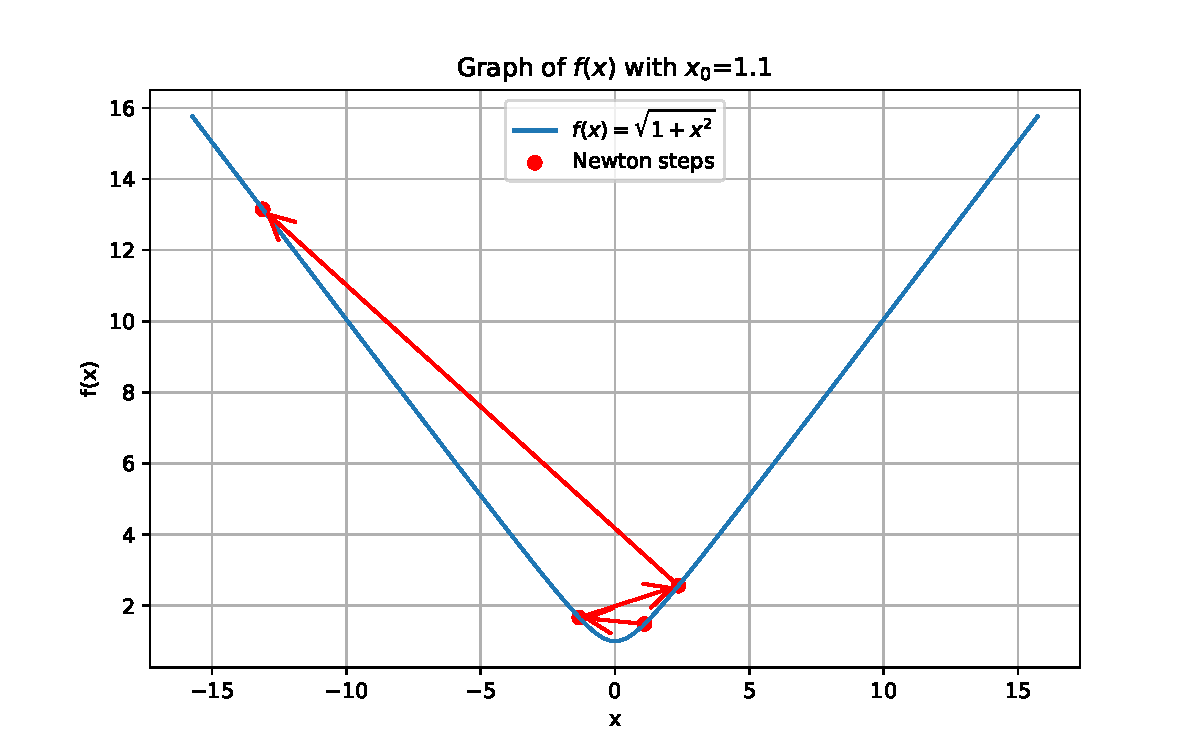
\includegraphics[width=0.6\textwidth]{../imgs/quasi_newton/newton_failure_sqrt_function_1.1.pdf}
    \caption{
        \ifEn
            An example where Newton's method diverges with initial point $x_0=1.1$
        \else
            初期点 $x_0=1.1$ でニュートン法が発散する例
        \fi
    }
    \label{fig:newton_failure_sqrt_function}
\end{figure}

\ifEn
    \paragraph{Oscillation of Newton's Method for Strongly Convex Functions}
\else
    \paragraph{強凸関数に対するニュートン法の振動}
\fi

\ifEn
    In the previous example, the objective function was not strongly convex and did not necessarily possess favorable properties.
    However, even for functions with the strong convexity property, there exist examples where Newton's method fails to converge \citep[Example 1.4.3]{Doikov2021SecondOrderTensor}.

    In this example, for $\mu>0$, consider the function
\else
    前の例では目的関数は強凸ではなく、必ずしも良い性質を持っていなかった。
    しかし、強凸性を持つ関数であってもニュートン法が収束しない例が存在する \citep[Example 1.4.3]{Doikov2021SecondOrderTensor}。

    この例では $\mu>0$ に対し、次の関数を考える。
\fi
\begin{align*}
    f(x)     & = \log(1 + e^x) - \frac{x}{2} + \frac{\mu x^2}{2}, \\
    f'(x)    & = \frac{e^x}{1+e^x} - \frac{1}{2} + \mu x,         \\
    f''(x)   & = \frac{e^x}{(1+e^x)^2} + \mu,                     \\
    f'''(x)  & = \frac{e^x(1 - e^x)}{(1+e^x)^3},                  \\
    f''''(x) & = \frac{e^x(1 - 4e^x + e^{2x})}{(1+e^x)^4}.
\end{align*}
\ifEn
    This function has the following properties:
\else
    この関数は次の性質を持つ。
\fi
\begin{enumerate}[nosep,label=\textbullet]
    \ifEn
    \item It is $\mu$-strongly convex.
    \item $\max_x |f''(x)| = \frac{1}{4} + \mu$ (attained at $e^x=1$). Hence, $\nabla f$ is $L$-smooth with $L=\frac{1}{4}+\mu$.
    \item $\max_x |f'''(x)| = \frac{1}{6\sqrt{3}}$ (attained at $e^x=2-\sqrt{3}$). Hence, $\nabla^2 f$ is $M$-Lipschitz with $M=\frac{1}{6\sqrt{3}}$.
          \else
    \item $\mu$-強凸である。
    \item $\max_x |f''(x)| = \frac{1}{4} + \mu$ であり、これは $e^x=1$ で達成される。したがって $\nabla f$ は $L=\frac{1}{4}+\mu$ の $L$-平滑である。
    \item $\max_x |f'''(x)| = \frac{1}{6\sqrt{3}}$ であり、これは $e^x=2-\sqrt{3}$ で達成される。したがって $\nabla^2 f$ は $M=\frac{1}{6\sqrt{3}}$ の $M$-Lipschitz である。
          \fi
\end{enumerate}
\ifEn
    Nevertheless, when the initial point $x_0$ is sufficiently large relative to $\mu$, Newton's method exhibits oscillatory behavior, as shown in \cref{fig:newton_failure_strongly_convex_function}.
\else
    それにもかかわらず、初期点 $x_0$ が $\mu$ に対して十分大きい場合、\cref{fig:newton_failure_strongly_convex_function} に示すようにニュートン法は振動する。
\fi

\begin{figure}[t]
    \begin{minipage}{0.5\textwidth}
        \centering
        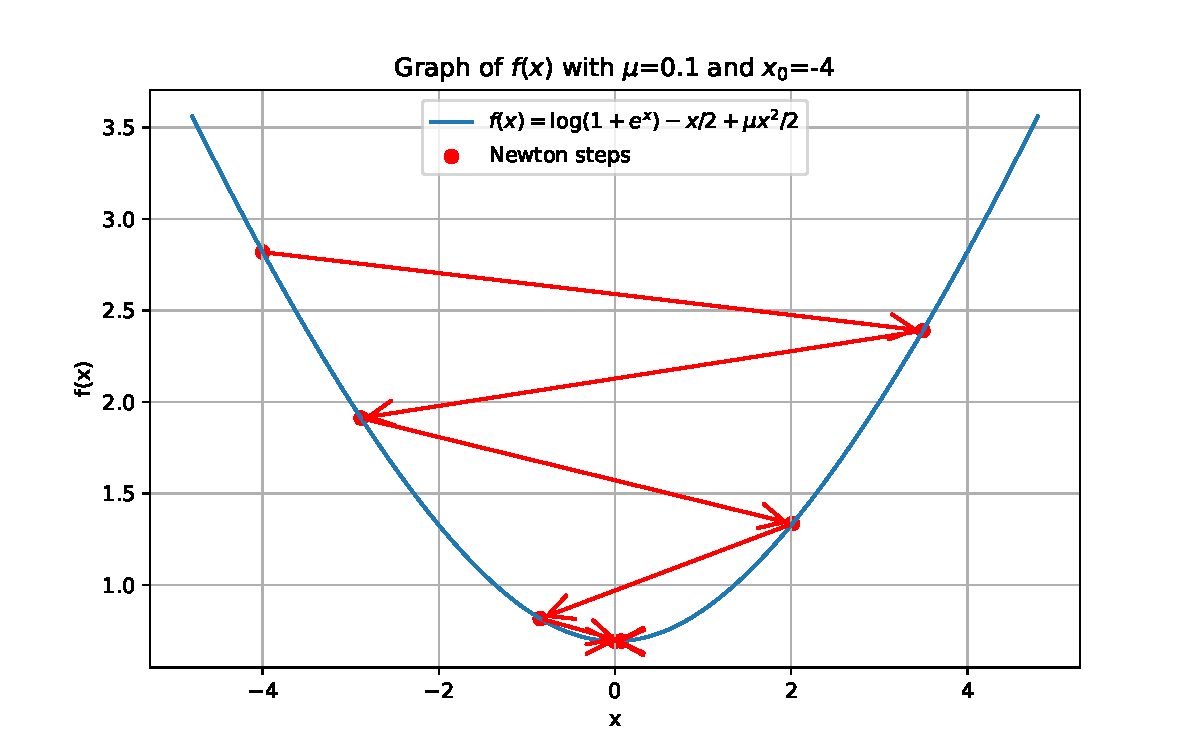
\includegraphics[width=\textwidth]{../imgs/quasi_newton/newton_failure_strongly_convex_function_0.1_-4.pdf}
    \end{minipage}%
    \begin{minipage}{0.5\textwidth}
        \centering
        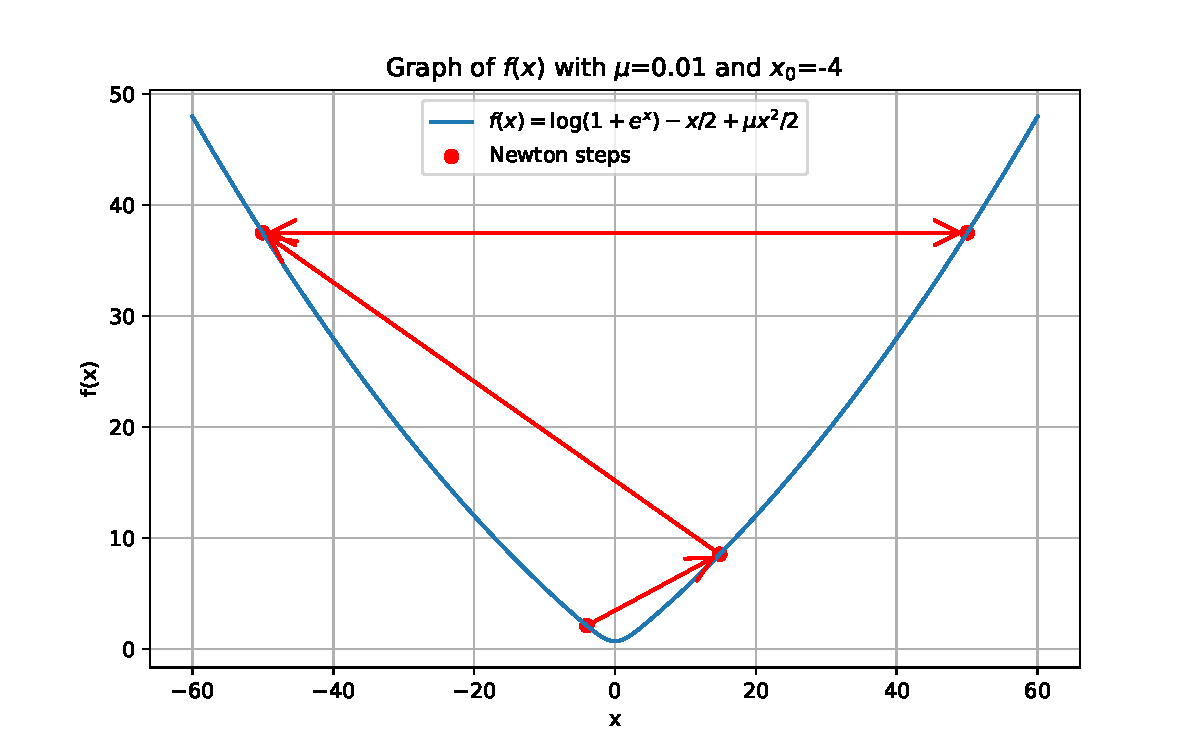
\includegraphics[width=\textwidth]{../imgs/quasi_newton/newton_failure_strongly_convex_function_0.01_-4.pdf}
    \end{minipage}
    \caption{
        \ifEn
            (Left) Newton's method converges for $x_0=-4, \ \mu=0.1$; (Right) Newton's method oscillates for $x_0=-4, \ \mu=0.01$
        \else
            (左) $x_0=-4, \ \mu=0.1$ ではニュートン法が収束する。(右) $x_0=-4, \ \mu=0.01$ ではニュートン法が振動する。
        \fi
    }
    \label{fig:newton_failure_strongly_convex_function}
\end{figure}

\ifEn
    \paragraph{Necessity of Line Search}
\else
    \paragraph{線形探索の必要性}
\fi

\ifEn
    To avoid the issues described above, it is common practice to select the step size $\alpha_k$ appropriately using a line search.
    Newton's method equipped with line search is often referred to as the modified Newton method and is known to possess global convergence properties.
\else
    上記の問題を避けるため、線形探索を用いてステップサイズ $\alpha_k$ を適切に選ぶことが一般的である。
    線形探索を備えたニュートン法は修正ニュートン法と呼ばれることが多く、大域収束性を持つことが知られている。
\fi

\ifEn
    \subsection{Comparison with Newton's Method as a Root-Finding Algorithm}
\else
    \subsection{根探索としてのニュートン法との比較}
\fi

\ifEn
    As a conceptual supplement, we briefly clarify the relationship between “Newton's method as a root-finding algorithm” and “Newton's method in optimization.”
    These two formulations are closely related, but they have different perspectives and applications.
\else
    概念的な補足として、「根探索としてのニュートン法」 と 「最適化におけるニュートン法」 の関係を簡潔に整理する。
    両者は密接に関係するが、視点と適用対象が異なる。
\fi

\ifEn
    \subsubsection{Newton's Method as a Root-Finding Algorithm}
\else
    \subsubsection{根探索としてのニュートン法}
\fi

\ifEn
    When referring simply to Newton's method (or the Newton--Raphson method), one often means a root-finding algorithm for a differentiable scalar function $g\colon \mathbb{R} \to \mathbb{R}$ that solves $g(x) = 0$.
    Although this is not the main topic of this section, it is arguably more fundamental and widely known.
\else
    単にニュートン法(あるいはニュートン・ラフソン法)と言うときは、微分可能なスカラー関数 $g\colon \mathbb{R} \to \mathbb{R}$ に対して $g(x) = 0$ を解く根探索アルゴリズムを指すことが多い。
    これは本節の主題ではないが、より基本的で広く知られている。
\fi

\ifEn
    Starting from an initial value $x_0$, the iteration is given by
\else
    初期値 $x_0$ から開始すると反復は次式で与えられる。
\fi
\begin{equation*}
    x_{k+1} = x_k - \frac{g(x_k)}{g'(x_k)}.
\end{equation*}
\ifEn
    Geometrically, this corresponds to approximating the graph of $g$ near $x_k$ by its tangent line and selecting the intersection of this tangent with the $x$-axis as the next approximate solution.
\else
    幾何学的には、$x_k$ 近傍での $g$ のグラフを接線で近似し、その接線と $x$ 軸の交点を次の近似解として選ぶことに対応する。
\fi

\ifEn
    \subsubsection{Newton's Method in Optimization}
\else
    \subsubsection{最適化におけるニュートン法}
\fi

\ifEn
    In the context of optimization, Newton's method typically refers to an algorithm for finding a local minimizer of a twice-differentiable function $f\colon \mathbb R^{n} \to\mathbb{R}$, or equivalently, a stationary point satisfying $\nabla f(x) = 0$ as a necessary condition.
    This is the primary focus of the present section.
\else
    最適化の文脈でのニュートン法は、二回微分可能な関数 $f\colon \mathbb R^{n} \to\mathbb{R}$ の局所最小点、または同値に必要条件 $\nabla f(x) = 0$ を満たす停留点を求めるアルゴリズムを指す。
    これが本節の主題である。
\fi

\ifEn
    Recall the assumption that the Hessian matrix $\nabla^2 f(x)$ is positive definite at each iteration.
    Newton's method in optimization applies the framework of the root-finding algorithm to the gradient $\nabla f(x)$:
\else
    各反復でヘッセ行列 $\nabla^2 f(x)$ が正定値であるという仮定を思い出そう。
    最適化におけるニュートン法は、根探索の枠組みを勾配 $\nabla f(x)$ に適用する。
\fi
\begin{equation*}
    x_{k+1} = x_k - \nabla^2 f(x_k)^{-1} \nabla f(x_k).
\end{equation*}
\ifEn
    In the scalar case, this reduces to $x_{k+1}=x_k - f'(x_k) / f''(x_k)$.
\else
    スカラーの場合、これは $x_{k+1}=x_k - f'(x_k) / f''(x_k)$ に簡約される。
\fi

\ifEn
    \subsubsection{Relationship Between the Two Formulations}
\else
    \subsubsection{二つの定式化の関係}
\fi

\begin{figure}[t]
    \centering
    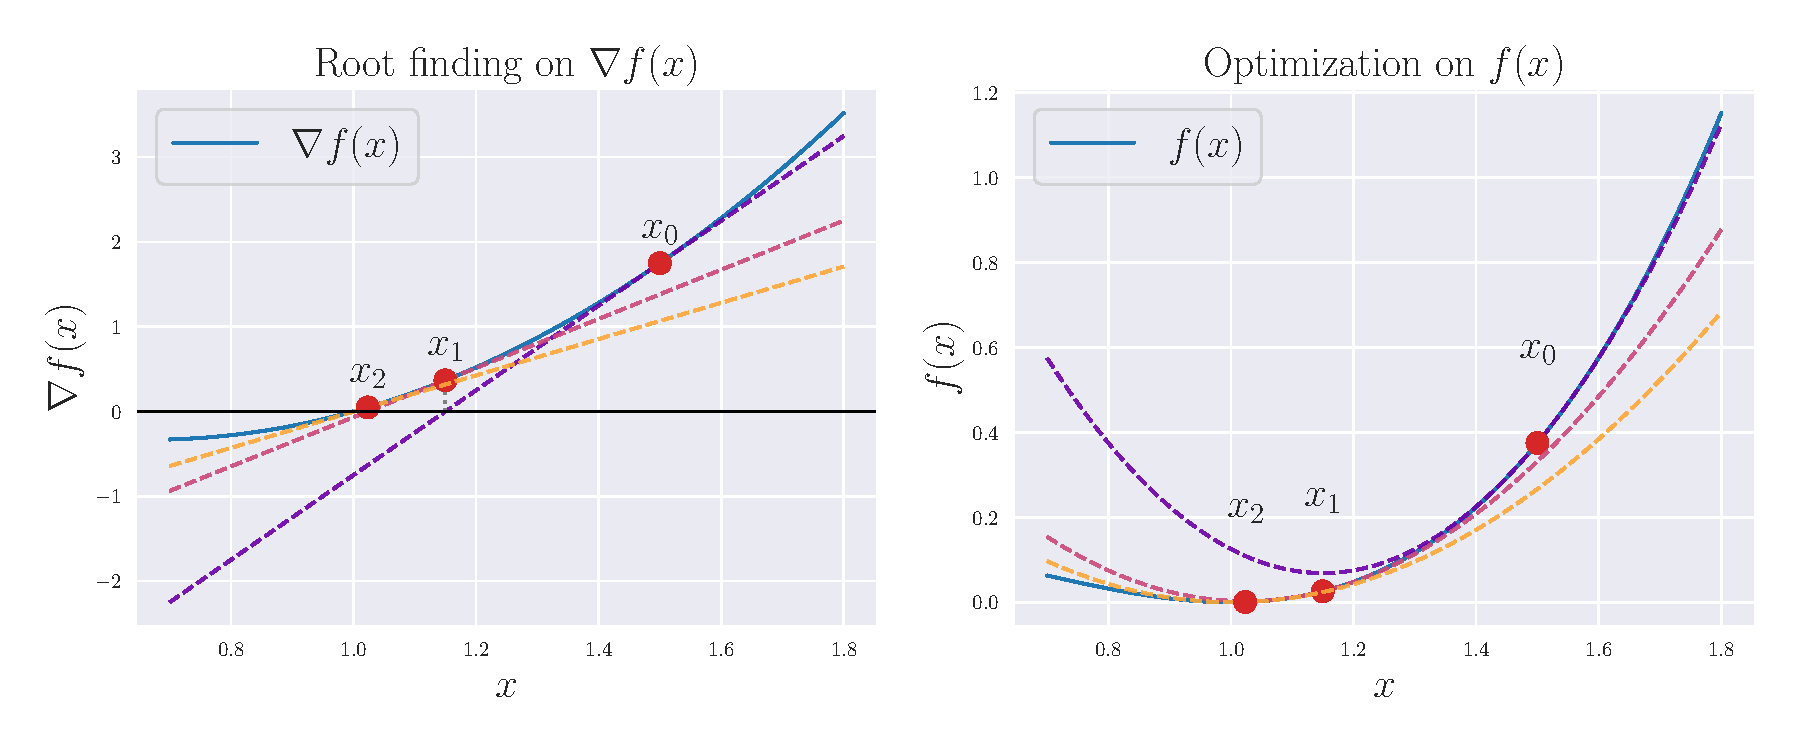
\includegraphics[width=\textwidth]{../imgs/quasi_newton/newton_raphson.pdf}
    \caption{
        \ifEn
            Root-finding for the gradient $\nabla f(x)=3 x^2 - 4 x + 1$ and optimization of the function $f(x)=x^3 - 2 x^2 + x$
        \else
            勾配 $\nabla f(x)=3 x^2 - 4 x + 1$ の根探索と関数 $f(x)=x^3 - 2 x^2 + x$ の最適化
        \fi
    }
    \label{fig:newton_raphson}
\end{figure}
\ifEn
    Let us examine the equivalence of the two formulations through a concrete example.
    \Cref{fig:newton_raphson} illustrates the relationship between these formulations using a simple cubic function $f(x)$.
    The left panel shows root-finding applied to $g(x) = \nabla f(x)$, while the right panel shows optimization applied to $f(x)$.
\else
    具体例を通じて両者の等価性を確認しよう。
    \Cref{fig:newton_raphson} は単純な三次関数 $f(x)$ を用いて両者の関係を示している。
    左図は $g(x) = \nabla f(x)$ に対する根探索であり、右図は $f(x)$ に対する最適化である。
\fi

\ifEn
    In the root-finding formulation, $\nabla f(x) = 3x^2 - 4x + 1$ is approximated by its tangent line, namely
\else
    根探索の定式化では、$\nabla f(x) = 3x^2 - 4x + 1$ を接線で近似し、すなわち
\fi
\begin{equation*}
    \nabla m^*_k(x) = \nabla f(x_k) + \nabla^2 f(x_k)(x - x_k),
\end{equation*}
\ifEn
    and the root of this linear model is chosen as $x_{k+1}$.
\else
    この線形モデルの根を $x_{k+1}$ として選ぶ。
\fi

\ifEn
    In contrast, in the optimization formulation, $f(x) = x^3 - 2x^2 + x$ is approximated by its second-order Taylor expansion
\else
    一方、最適化の定式化では、$f(x) = x^3 - 2x^2 + x$ を二次のテイラー展開で近似し、
\fi
\begin{equation*}
    m^*_k(x) = f(x_k) + \nabla f(x_k)(x - x_k) + \frac{1}{2}\nabla^2 f(x_k)(x - x_k)^2,
\end{equation*}
\ifEn
    and the minimizer of this quadratic model is taken as $x_{k+1}$.
\else
    この二次モデルの最小点を $x_{k+1}$ とする。
\fi

\ifEn
    Thus, under the assumption of positive definiteness, it is clear from the properties of local solutions that both formulations perform essentially equivalent operations, and their correspondence can be explicitly verified.
\else
    したがって、正定値性の仮定のもとでは局所解の性質から両者が本質的に等価な操作を行うことが分かり、その対応関係を明示的に確認できる。
\fi

\ifSubfilesClassLoaded{
    \bibliographystyle{plainnat}
    \bibliography{../L-BFGS.bib}
}{}

\end{document}
